\begin{figure*}[htbp]
    \centering
    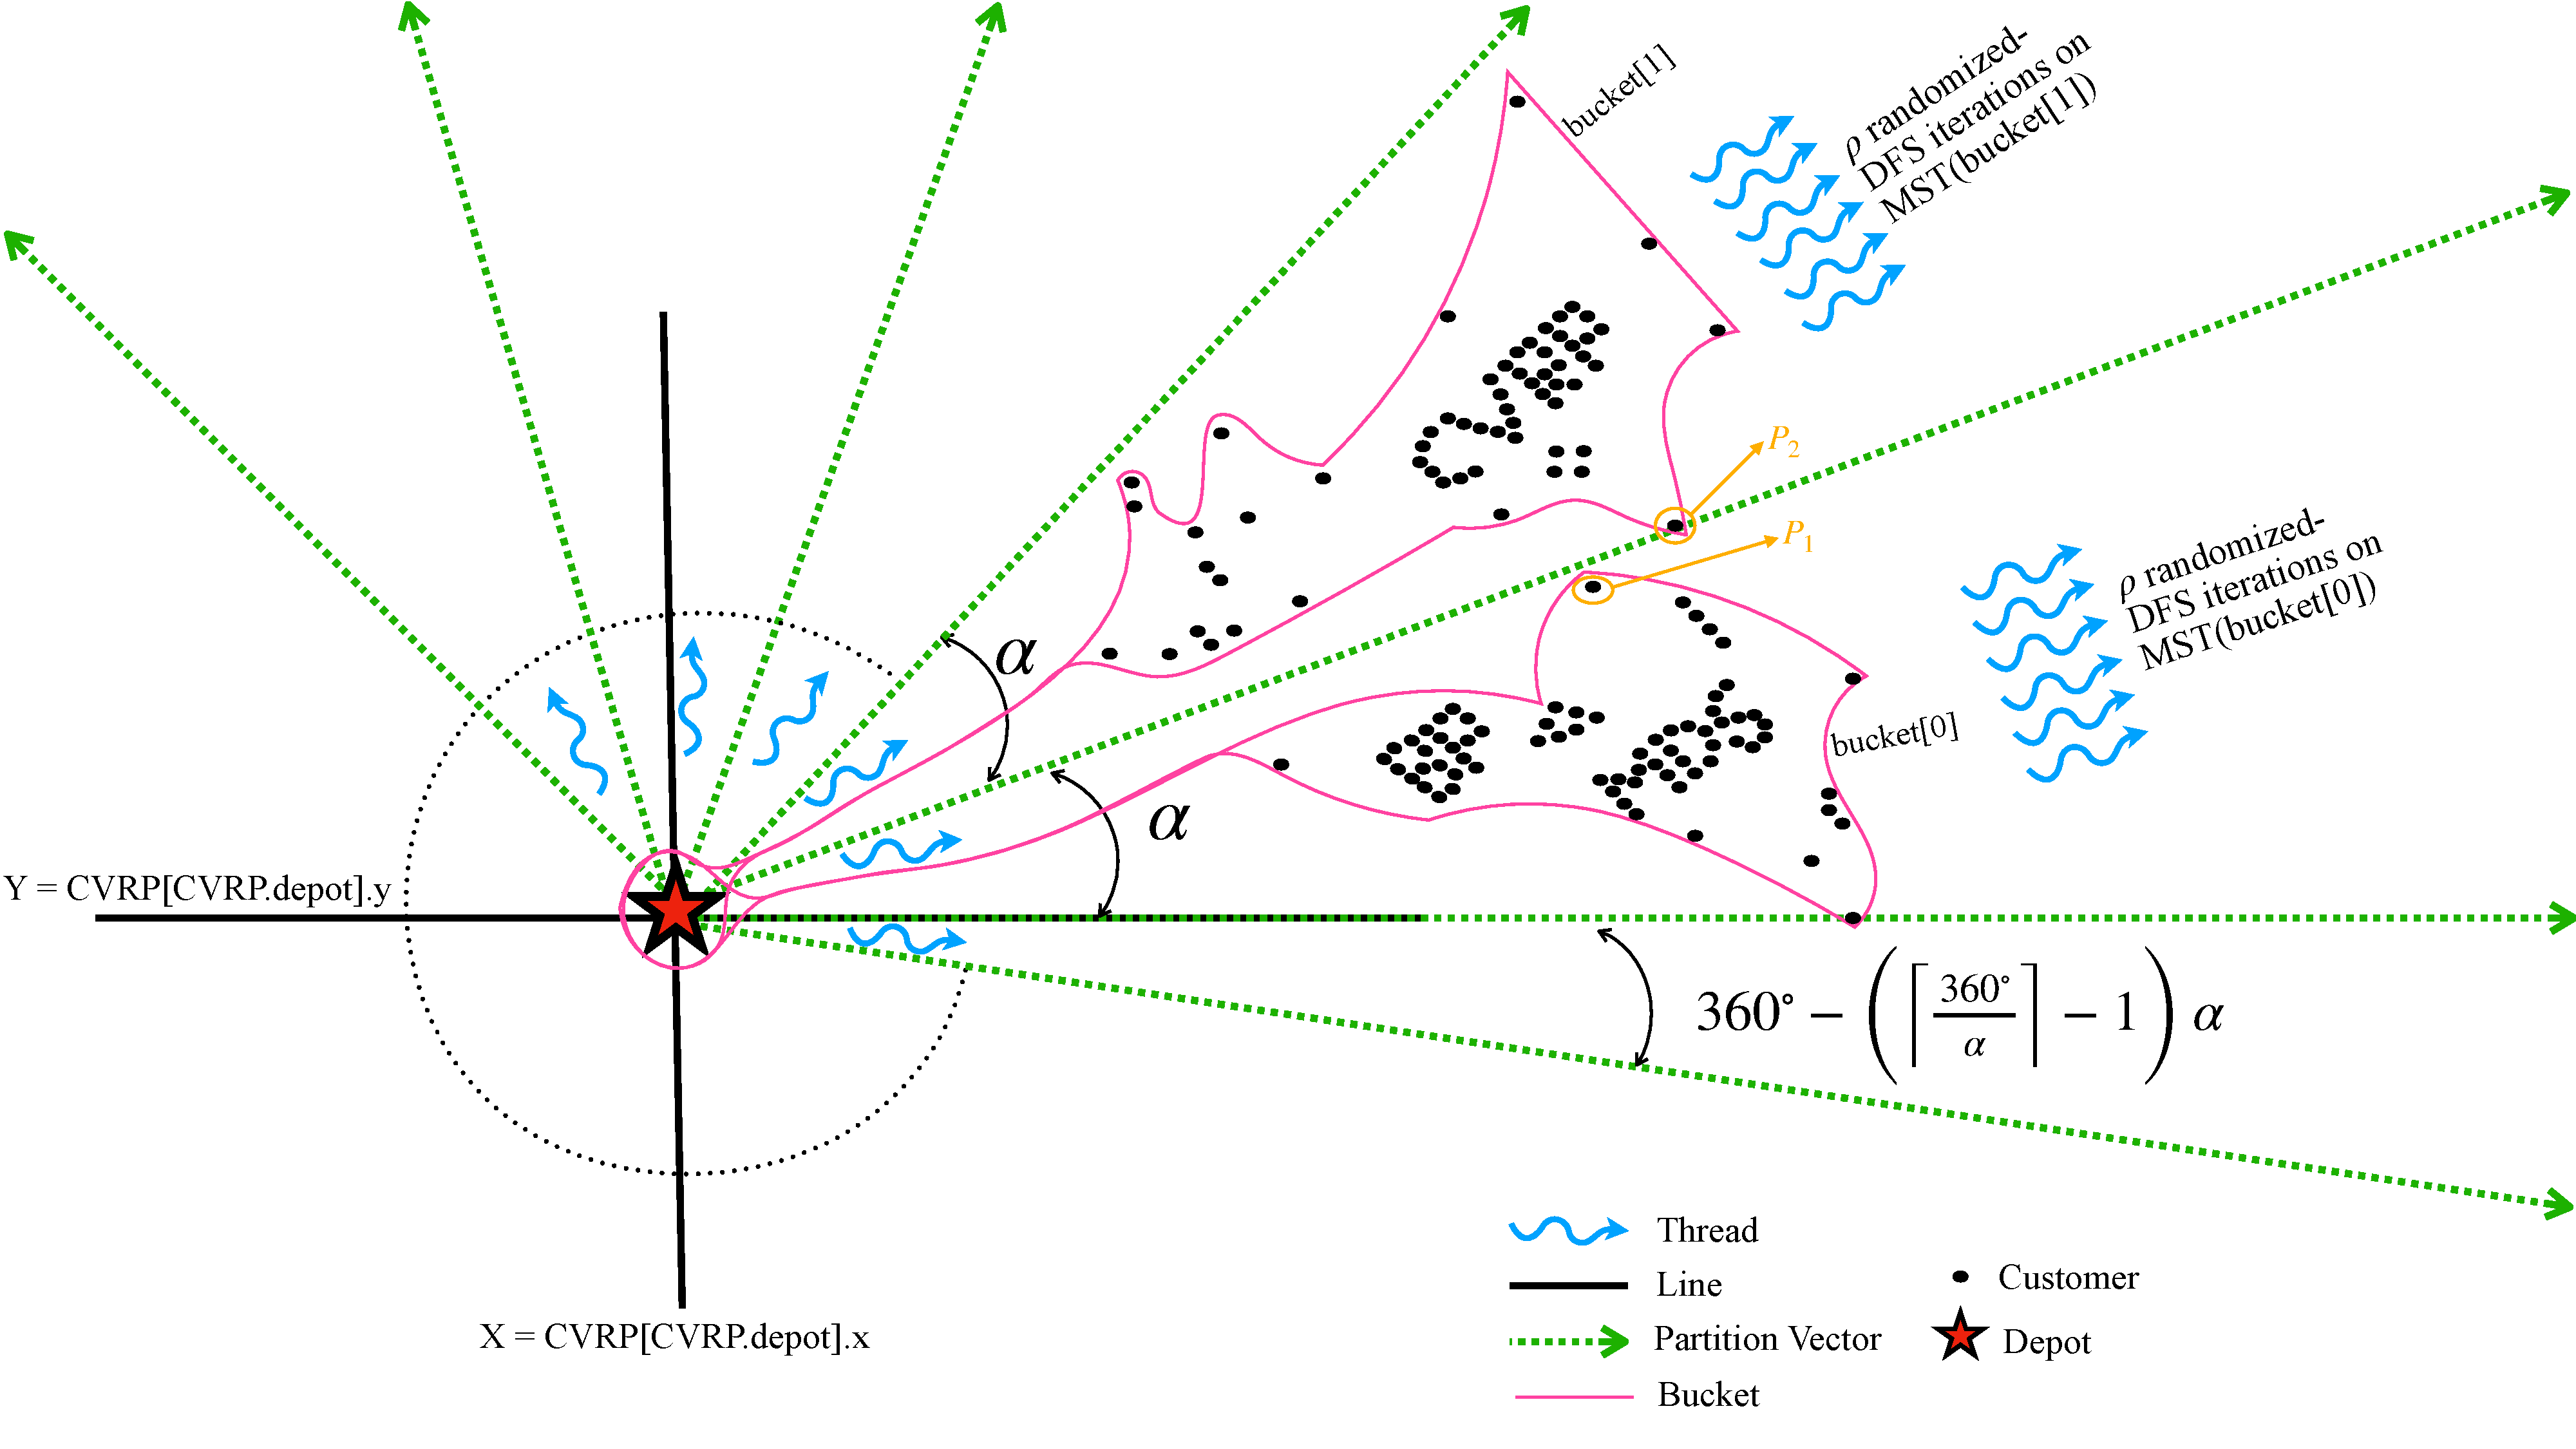
\includegraphics[width=\textwidth, height=0.45\textheight, keepaspectratio]{assets/2-d-partitions-refined.pdf}
    \caption{2-D partitioning in BP-MDS}
    \label{fig:2-d-partition}
\end{figure*}

\section{Background and Related Work}
\label{sec::background}

In CVRP, we are given a depot and $(N-1)$ customer nodes. Each node $id \in \{0, 1, \dots, \allowbreak N-1\}$ is associated with coordinates\\$(CVRP[id].x,\allowbreak\ CVRP[id].y)$ in the 2D Euclidean plane, where the depot is identified by $id = 0$. Each customer node $id$ has an associated demand $CVRP[id].demand$ satisfying $0 < CVRP[id].demand \leq Q$, where $Q$ denotes the capacity of each vehicle. The depot has zero demand. A fleet of identical vehicles, each with capacity $Q$, is stationed at the depot, and the fleet size is assumed to be sufficiently large to serve all customers. The cost between any pair of nodes is defined as the Euclidean distance between their corresponding coordinates. The objective is to determine a set of routes such that each route starts and ends at the depot, each customer is visited exactly once, and the total demand served in any route does not exceed the vehicle capacity $Q$, while minimizing the total travel cost. A CVRP instance can be modeled as a complete weighted graph $G = (V, E)$, where $V$ denotes the set of nodes, $E$ the set of edges, and edge weights represent pairwise distances between nodes.

State-of-the-art solutions for medium-scale CVRP instances are typically obtained using metaheuristics such as Genetic Algorithms, Tabu Search, and Hybrid Genetic Search (HGS)~\cite{vidal2012hybrid}, which are highly effective in reducing the optimality gap and often achieve near-optimal solutions. A significant body of research has also focused on designing heuristic and metaheuristic approaches that trade optimality for computational efficiency~\cite{Toth_VRP}, including classical methods such as the Clarke--Wright savings algorithm~\cite{Clarke_Wright} and sweep-based heuristics~\cite{Sweep_Heuristic}, which exploit geometric properties to construct feasible routes efficiently. More recent advances combine local search with powerful diversification strategies to further improve solution quality~\cite{vidal2022hybrid}. However, despite their effectiveness on benchmark datasets, these approaches remain computationally intensive and exhibit limited scalability when applied to instances with hundreds of thousands or millions of nodes, with execution time and memory requirements posing significant challenges.

With the rise of multi-core and high-performance computing systems, parallel approaches to CVRP have gained traction. These methods distribute either the search process or the problem structure across processing units. Crainic~\cite{crainic2006parallel} introduced an early and influential parallel metaheuristic that explores multiple solution trajectories concurrently. Despite their effectiveness, such approaches often incur synchronization overhead and exhibit limited scalability due to shared data structures. Tree-based heuristics, especially those based on Minimum Spanning Trees (MSTs), are widely used in routing due to their ability to capture the graph structure efficiently. MST-based methods are computationally light and often serve as a backbone for constructing feasible tours~\cite{CLRS}. Combining spanning trees with traversal strategies such as depth-first search~(DFS) enables the generation of approximate solutions with linear or near-linear time and low memory overhead, making them suitable for large-scale instances. ParMDS~\cite{Muniasamy_VRP} follows this paradigm by constructing an MST over the complete CVRP graph and exploring multiple randomized DFS traversals to generate diverse route sets. While effective, its scalability is limited to approximately $5\times 10^4$ customers in the input instance.

Our work builds upon these directions by combining spatial decomposition with tree-based route construction in a parallel setting. Unlike classical metaheuristics that focus on solution optimality, our primary objective is to achieve scalable performance on massive CVRP instances. Compared to ParMDS~\cite{Muniasamy_VRP}, our approach introduces a lightweight angular partitioning scheme coupled with randomized exploration over MST structures, enabling efficient utilization of modern multi-core architectures. The proposed Bucket-Partitioned-MDS (BP-MDS) framework is designed to balance solution quality, execution time, and memory usage, making it suitable for million-scale CVRP instances where traditional methods become impractical. Unlike single-threaded solvers such as \textsc{HGS-CVRP}, which primarily prioritize solution quality and are typically limited to instances with a few thousand customers, our proposed \textsc{BP-MDS} scales to million-customer problem instances and delivers orders-of-magnitude speedups.

